\documentclass[a4paper]{article}
\usepackage{natbib}
\usepackage{booktabs}

%% Language and font encodings
\usepackage[english]{babel}
\usepackage[utf8x]{inputenc}					% for using international characters
\usepackage[T1]{fontenc}						% proper font encoding
%\usepackage[babel=true]{microtype}				% better looking text
%\usepackage{lmodern}							% since fontenc changes the font, we want to change is back

%% Sets page size and margins
\usepackage[a4paper,top=3cm,bottom=2cm,left=3cm,right=3cm,marginparwidth=1.75cm]{geometry}

%% Useful packages
\usepackage[colorinlistoftodos]{todonotes}
\usepackage[gen]{eurosym}						% Euro symbol
\usepackage{amsmath,amsfonts,amsthm,amssymb}
\usepackage{latexsym,graphicx}
\usepackage{dsfont}
%\usepackage{verbatim}							% for verbatim prints like matlab code etc
%\usepackage{mathrsfs}							% script fonts in maths
%\usepackage{bm}								% bold symbols and bold math mode
\usepackage{color}
\usepackage[colorlinks=true, allcolors=blue, breaklinks=true]{hyperref}
%\usepackage{url}
\usepackage{multirow,bigstrut}					% tables with multirows
\usepackage{multicol}
\usepackage{subcaption}

%% For Drawing
\usepackage{tikz}								% for drawing
\usetikzlibrary{shapes.geometric, arrows}
\tikzstyle{box} = [rectangle, minimum width=3cm, minimum height=1cm, text centered, draw=black, text width=3cm]% fill=orange!30
\tikzstyle{box2} = [rectangle, minimum width=2cm, minimum height=1cm, text centered, draw=black, text width=2cm]% fill=orange!30
\tikzstyle{arrow} = [thick,->,>=stealth]

%% Colors
\definecolor{rred}{RGB}{204,0,0}
\definecolor{ggreen}{RGB}{0,145,0}
\definecolor{yyellow}{RGB}{255,185,0}
\definecolor{bblue}{rgb}{0.2,0.2,0.7}
\definecolor{ggray}{RGB}{190,190,190}
\definecolor{ppurple}{RGB}{160,32,240}
\definecolor{oorange}{RGB}{255,165,0}


%% Definitions
\newtheorem{hypothesis}{Hypothesis}


%% Multiple author package
\usepackage{authblk}

\title{Assessing Upstream Supply Chains Through Physical and Amplifying Water Risk Indicators.}
\author{Torben Schaefer}
\author{Maximiliano Udenio\thanks{m.udenio@tue.nl} }
\author{Shannon Quinn}
\author{Jan C. Fransoo}

\affil{Department of Industrial Engineering, Eindhoven University of Technology, 5600 MB Eindhoven, The Netherlands}

\date{}

\begin{document}
\sloppy % this command solves the overfull paragraphs with citations not breaking

\maketitle

\begin{abstract}
Although sustainability has long been recognized as a fundamental practice in manufacturing, and firms have been devoting resources to reduce their carbon footprint, greenhouse gas emissions, and water use, the problem of measuring and acting upon water risk in the supply chain has not yet been tackled in the literature. 
Unlike other environmental concerns, water risk is a local phenomenon that needs to be quantified at the catchment level.  
Thus, the impact of a production process cannot be generalized and must be analyzed within its particular context---ideally at the production site level.
Furthermore, recent trends in manufacturing (such as ``local production'') are expected to put increased pressure in areas where regulations are lax and water risk is high (e.g., India, China).
Such considerations can be taken into account within the context of supplier selection.
We introduce a hierarchical framework to quantify and aggregate relevant water risk indicators into an index score designed to assess suppliers' water risk based on their location. 
Our framework distinguishes between a higher-level identification of ``water-sensitive'' supply chains and the low-level assessment of the water risk at the regional/supplier/product level. 
We illustrate the application of our framework with a case study at a large multinational company. 
We show two applications of particular importance for managers: bottom-up study of supplier selection at a raw-material level, and top-down identification of country-level aggregate risk and variability.
\end{abstract}

\section{Introduction}
April 2016, Mumbai---India. 
Water scarcity in the Maharashtra province pushed civic bodies to interrupt water flows to industrial belts. 
Experts estimate that this decision had a negative effect on India's index of industrial production growth (IIPG) on the order of 40 to 50 basis points (0.4--0.5\%), with the manufacturing sector alone taking a hit of 50 to 75 basis points (0.5--0.75\%) (REF).
July 2016, Cochabamba---Bolivia. 
159 out of the city's 300 industries experienced production interruptions due to a water shortage caused by droughts. 
30 municipalities declared a state of emergency. 
xxx estimated that industrial production in the area decreased 15\% (REF). 
March 2017, Arequipa---Peru. 
Floods and mudslides followed intense rains in the south of the country. 
Water quality in the area suffered; the abnormal murkiness of the fresh water supply made sanitation impossible. 
Thousands of people and dozens of industries lost regular access to clean water for weeks (REF).


Climate change has disrupted previously stable cycles of rain, snow, and storms, making the natural supply of fresh water unpredictable (REF). 
The relative speed of the transition to such unstable global water conditions has surprised governments and companies alike \citep{Schneider:2016}.
Recent studies indicate that at least four billion people face severe water scarcity at least one month a year \citep{Mekonnen:2016}.
As the above examples illustrate, industrial locations--sharing water resources with civilian populations--are particularly sensitive; disruptions in the water flow typically force production shutdowns.
Infrastructure deficiency, regulations, and growth in water demand contribute to the fact that water is becoming a scarce resource in many regions around the world \citep{OECD:2011, Schyns:2015}. 
Moreover, this view of water as a scarce resource, and the subsequent competition for its use, is expected to increase in the future \citep{Hoekstra:2014, WEF:2015}.
As a result, water scarcity has been identified as one of the top global sustainability risks today. 

Formally, water scarcity is defined as \textit{``an excess of water demand over available supply''} \citep[][p.xx]{Steduto:2012}.
With respect to demand, water requirements increased at a rate more than double than that of the population increase during the past century \citep{Zabarenko:2011}.
With respect to supply, water is a renewable resource, but its availability is limited. 
It is a finite resource; there is a limited amount of precipitation, and water has to run through the hydrologic cycle before becoming available again \citep{Hoekstra:2013,Schyns:2015}.
Water, moreover, is a local resource distributed unequally around the globe; as are the quality of local regulatory frameworks and infrastructure. 

Water is a key ingredient in the manufacturing operations of a large number of firms \citep{Jones:2014}. 
Due to the increasing water challenges, investors increasingly expect firms to assess their internal and external water risks. 
Organizations such as the Carbon Disclosure Project (CDP), allow firms to disclose sustainability information and have extended their scope to include water risks \citep{CDP:2015}.
Other firms have adopted corporate water stewardship (CWS, REF).
Therefore, firms with significant water requirements generally track their internal water use in production as well as during the use phase of their finished products.
Such measurements enable firms to quantify the impact of their processes on water use \citep{Hoekstra:2016} or water scarcity \citep{Pfister:2017}.
%Consequently, firms use water-risk assessment methodologies to identify vulnerable sites from both manufacturing and usage perspectives. 
Nevertheless, the number of firms reporting and using such data is still small. 
Based on the latest CDP report: ``while more than two-thirds of supplier respondents to the supply chain program saw climate change opportunities, only 36\% of suppliers responding to CDP’s water program identied water-related opportunities. And only 28\% see any water risks to their business, which compares to three-quarters that see climate change risks.'' \citep{CDP:2017}.

The problem of assessing the impact of water usage in the upstream supply chain (i.e., a firm's suppliers, their suppliers, and so on), however, has not been addressed in the literature thus far. 
This is despite that, often, a significant portion of the total environmental impact of a firm can be attributed to processes upstream \citep{Pelton:2016}.
As transparency of suppliers gains importance for competitiveness (REF), firms must extend their water-risk management methodologies to their upstream partners.
%Assessing such risks, however, is a complex exercise. 

%Sustainability initiatives for water are typically established under the Corporate Water Stewardship (CWS) domain.
%CWS concerns the sustainable managing of a firm's water resources among different stakeholders; suppliers, governments, and consumers \citep{Orr:2011}.
%To implement overarching measures to reduce water risk at a supply chain level, continuous monitoring at the local level is needed. 
%In the case of large multinational firms, working with hundreds or thousands of suppliers, the scale of this challenge is enormous \citep{Environ:2015}.

We argue that, compared to other sustainability areas, three main factors make water risk management at a supply chain level a unique challenge going forward: (1) The local nature of water risk, implying that it must be measured at a micro level, thus at the level of individual manufacturing locations; (2) The  rise of developing economies such as India and China as major manufacturing centers for the global economy \citep{Friedman:2005} and in particular, the proliferation of specialized, small-scale, suppliers in industrial belts of these economies located in high water-risk areas; and (3) The clear hierarchy between water destined for human consumption and industrial use, whereupon water flow to factories is expected to be interrupted as demand for sanitized water outstrips supply in a particular area.    

%Water is a global resource with a local impact. 
%Its temporal unavailability and ecosystem impact resulting from its use on a given location is hard to predict. 
%Moreover, other local traits, such as government regulations and available infrastructure, further increase the complexity of a proper assessment.
%This is of particular importance for large manufacturing firms, whose suppliers can number in the thousands and be spread across the globe.
%Competition for limited water resources between the local population and the industry is a concern in densely populated, low income, areas.

In this paper, we develop a framework for water-risk screening in an upstream supply chain.
We are inspired by the risk management literature \citep{Sodhi:2012} and its application to sustainability research \citep{Giannakis:2016}. Furthermore, we position our study within the ``green supplier selection'' problem \citep{Appolloni:2014} by considering access to water as a location-level multi-dimension risk criteria. 
In our framework, we explicitly distinguish between the identification of vulnerable supply chains from the assessment of the water-risk of all suppliers. 
We use volumetric water footprint indicators for the former; the latter is accomplished through a theory-based set of risk indicators aggregated into a risk index through a Monte Carlo Analytic Hierarchy Process (MCAHP).

We illustrate the use of our framework through the analysis of upstream water risk on a multinational consumer goods firm. 
Our model singled out 14 suppliers out of over 1000 that have an increased future risk. 
(top-down approach.)
Moreover, we complement the use of our framework with product-level water consumption data to compare alternative suppliers for specific water-intensive raw materials. 
This allows us to quantify the water risk per at the site level.
(bottom-up approach.) 

This paper contributes to the theory by linking the issue of water risk with the supplier selection problem, with an eye to developing countries, where regulations are lax and water pressure is high. 
We also have a strong managerial contribution in the development of an easy-to-adopt tool that allows tactical decision making at a product-level, as well as a region-level. 

\section{Related Literature}
Since our main contribution is the development of a water risk screening framework within the area of risk management/supplier selection, we structure the discussion of related literature as follows.
In Section \ref{lit:supp_select} we discuss the issue of supplier selection; the methodologies employed and the most relevant articles. 
Next, in Section \ref{lit:SCRM}, we survey the literature related to supply chain risk management and, in particular, the literature discussing explicit sustainability-related risks. 
Finally, in Section \ref{lit:water} we identify the issue of water stewardship and its relevance to SCM.

We focus on the papers most relevant to our study.
We refer the reader to \citet{Tang:2006} and \citet{Scholten:2017} for in-depth reviews of supply chain risk, uncertainty, and their link to sustainability; \citet{Jaehn:2016} and \citet{Tang:2012}, for literature reviews on sustainable operations; \citet{Ho:2010} and \citet{Chai:2013} for reviews on decision-making techniques on supplier selection; and \citet{Appolloni:2014} for a review of green procurement in the private sector. 



\subsection{Supplier Selection and Supplier Management}\label{lit:supp_select}
Supplier Selection (SS) and Supplier Management (SM) refer to the systematic decision making strategies behind choosing, monitoring, and developing suppliers.

The first step in any SS problem is to define a set of criteria with which to evaluate suppliers.
These criteria vary, and can be quantitative (e.g., liquidity, revenue) as well as qualitative (e.g., social responsibility) (REF). 
Following this, several techniques are used to quantify the criteria and rank the suppliers. 
In the field of decision making theory, the techniques typically applied in SS can be clustered into three main categories: Multicriteria Decision Making (MCDM), Mathematical Programming (MP), and Artificial Intelligence (AI).
\citet{Chai:2013} find that, of the 123 journal articles published on the topic between 2008 and 2013, the majority (62\%) used MCDM techniques, followed by MP (49\%), and AI (29\%)\footnote{Note that a number of papers use multiple techniques from multiple categories}. 
Analytic Hierarchy Process (AHP), a type of MCDM, is the single most common technique, appearing in 25\% of all articles surveyed.
Other popular techniques are Linear Programming (MP, 15\%), TOPSIS (MCDM, 15\%), and Analytic Network Process (MCDM, 12\%). 

Sustainable supplier selection incorporates sustainability-derived criteria into the problem.
For example, \citet{Hashemi:2013} use AHP to present an integrated framework for green supplier selection. 
The authors integrate criteria such as resource consumption and pollution production into the SS problem and perform a case study in an automobile factory. (put one or two more examples here.)

A natural extension of SS is Supplier Management (SM), where the scope is expanded to include monitoring and developing existing buyer-supplier relationships \citep{Modi:2007, Ivens:2013}.
Methodologically, the monitoring of suppliers follows the SS process \citep{Ittner:1999}; the development of suppliers, however, is triggered by the evaluation of suppliers at either the selection or monitoring stage \citep{Hahn:1990}.
Given that firms usually deal with a large number of diverse suppliers, a common strategy is to identify the most important relationships to work on, i.e., key supplier management \citep{Ivens:2009}. 
See \citet{Vijver:2009} for a complete review of the literature on collaboration on buyer-supplier relationships. 

As with SS, the extension of SM into sustainable SM corresponds to the inclusion of sustainability as a metric to monitor and develop the existing buyer-supplier relationships.
\citet{Zimmer:2015} review the state of the sustainable supplier management literature. 
They identify 143 articles, published between 1997 and 2014, related to sustainable SM.
In line with the recent popularity of the field,  83\%  were published after 2010.
However, the majority (81\%) focus on supplier selection, neglecting post-selection steps. 
In terms of techniques, their findings are in line with \citet{Chai:2013}.% AHP, ANP, and TOPSIS being popular. 
In their classification, however, Fuzzy Logic (AI) is the most popular technique (31\%) followed by AHP (19\%).
They suggest that the reason behind the popularity of Fuzzy Logic is that it combines well with mathematical-analytical methods.
In terms of the identification of performance criteria according to their sustainability dimension, economic, environmental, and societal criteria make up, respectively, 53\%, 38\%, and 9\% of the total.
It is interesting to note that water-related criteria make up only 1.8\% of the total.


\subsection{Supply Chain Risk}\label{lit:SCRM}

Globalization and the increase in length and complexity of supply chains brought about a myriad of advantages, but also increased exposure to uncertainty (REF). 
As a result, supply chain risk management has emerged as a fast-growing research topic (REF).
Supply Chain Risk Management attempts to handle uncertain (and disruptive) events in a systematic way.

In their framework for supply chain risk management, \citet{Sodhi:2012} define three steps for SCRM: identify, assess, and mitigate (check).
In a supply chain, risk can take different forms. 
(REF) define SC risks as endogenous (i.e., caused by the internal SC structure) or exogenous (i.e., caused by external developments); and from the point of view of a firm operating within a SC, as supply-side or demand-side. 

While research exists focusing on methodologies for identification (REF), assessment (REF), and mitigation (REF) of risks; a large body of literature exists where the aim is to tackle a particular interest/industry/problem.
In this view, relevant risks are typically categorized on the frequency and impact dimensions. 
Low-likelihood, high-impact risks (REF) are generally modeled using xxx and solutions tend to include redundancy, fast response, etc.
High-likelihood, low-impact risks (REF), on the other hand, are found to be xxx and typically mitigated through a combination of yyy and zzz. 

In recent years, interest has appeared on sustainability-related SC chain risks \citep{Giannakis:2016}.
Rather than focusing exclusively on potential SC disruptions, this community is interested in classifying and assessing the environmental and societal risks associated with SCM. 
A number of articles argue that any risk management methodology needs to incorporate sustainability-related risks \citep{Cousins:2004, Teuscher:2006, Anderson:2006, Anderson:2009}. 
These authors, however, typically incorporate sustainability-related risks into the financially-based performance measurements common in SCRM. (As opposed to including sustainability itself as an explicit performance metric.)

\citet{Cousins:2004} introduce a framework where environment-related supplier initiatives act as a feedback loop for the analysis of the exposure of firms to risks (in the natural environment as well as business surroundings).
From a strategic perspective, they warn against the over-reliance on a single supplier that may have a negative impact on the environment, or that ``may fall foul of environmental legislation, regulation or public opinion''.
They classify environment-related supplier initiatives according to the level of perceived losses (i.e., high or low financial, societal, etc losses) and the availability of advanced strategic purchasing resources within a firm. 
Firms facing a similar threat will react differently according to their level of resources, and vice-versa. 

\citet{Anderson:2009} argue for mitigation of sustainability risk management citing figures from the British Government \citep{Stern:2007}: the cost of mitigating sustainability risks is estimated at approximately 1\% of the world's GDP, the potential costs related to adverse impacts are estimated at between 5\% and 20\% of the world's GDP. 
While these figures were subsequently disputed \citep{Weitzman:2007}, researchers broadly agree with the conclusion that sustainability actions can be justified on economic grounds \citep{Tol:2006}.

\citet{Giannakis:2016} recognize a number of similarities and differences between sustainability SCRM and ``typical'' SCRM. 
Sustainability-related risks are often easy to identify and difficult to assess. 
In part, this is due to the difficulty in assigning a quantitative value to factors such as long-term decline of the environment or of a firms' reputation. 
Nevertheless, the authors suggest that many sustainability-related risks can be considered as precursors of commonly studied risks such as supply or demand-side disruptions. 
This suggests that a framework for sustainability risk management can complement traditional SCRM.
In fact, they argue, sustainability risk management should be part of an overall strategy for risk management. 

\subsection{Water Footprinting and Stewardship}\label{lit:water}
We can split this section into three; the literature that looks into actual water usage (water footprinting), the literature that includes water into LCA-type inventory and impact analysis, and the literature that deals specifically with corporate decision-making based on water risks. 

Water Footprinting (WF, \citet{Hoekstra:2011}) started as a methodology to explicitly measure the impact of man-made processes on the availability of water. 
At its core, WF associates a volumetric use of water to a given process and a volumetric availability based upon the location of the process \citep{Hoekstra:2011}.
To quantify the effect of a given process on the environment, thus, WF uses the ratio of local demand to supply.
Also crucial for WF, the distinction between blue, green, and grey water. 
Blue water is the water from a catchment (water body); green water is the runoff water from rain; and grey water is the volume of water required to assimilate the load of pollutants.

The inventory activities of LCA are comparable to WF. 
That is, a volumetric measurement of water used by a process or product. 
LCA, however, differs in two important aspects from the philosophy of WF. 
First, only blue water is considered in its measurement. 
The reasoning is that it is the main water source for industrial applications.
Second, the proposed method to assess the local impact of a process is a water-scarcity weighted water footprint.

There are arguments defending both positions \citep{Hoekstra:2016, Pfister:2017}.
WF proponents \citep{Hoekstra:2016} argue that the LCA methodology distorts the real problem by introducing an artificial index that is not suitable for comparison across processes/locations.
Moreover, they also argue that conceptually the amount of water stress is irrelevant for measuring the sustainability of a process, i.e., as long as the demand of water in a certain location is lower than its supply, then the location is sustainable in terms of water use---irrespective of any other factors.
On the other hand, Hoekstra argues that even though water is a local resource, the impact should also be considered globally. 
In SC thinking, this means that when two alternative processes exist, then under a global view, as long as it is sustainable, the process with smaller volumetric impact is preferred. 
Even if it means extracting water from a more scarce area. 
\citet{Hoekstra:2016} cites an example where xxxx.    

LCA proponents \citep{Pfister:2017} retort that yyyy (fill paragraph).

Firms are aware of the water challenges of today and the future.
KPMG (2012) report that ``companies in all sectors need to prepare themselves for a world where raw materials may be in short supply and subject to price volatility including large price increases and increased disruption to supplies.''
In particular, \citet{Makower:2014} argues that water is, in the mind of consumers, governments, and firms alike, already associated with global risks and crises. (check that wording is consistent and add 2017 report.) 
Furthermore, KMPG (2012) defines water scarcity is one of the top ten sustainability ``megaforces'' that will impact every business in the coming decades.

Therefore, many firms have adopted the issue of water usage within corporate social responsibility/sustainability initiatives, under the moniker of water stewardship.
The alliance for water stewardship (2013) defines it as ``xxx''.
In a broader interpretation of the term, the World Wildlife Fund (2013) explicitly includes ``value chain operations'' within the scope of water stewardship. 
However, even as sustainability reporting is now expected from firms, and even as several guidelines targeting businesses are in place (e.g., the corporate water disclosure guidelines from the UN global compact (2014 REF) and xxx from the carbon disclosure project), current practice is unstructured and highly variable.
 
\citet{Jones:2014} conducted a study on the disclosure of water sustainability reports of the UK's ``top twelve superbrands''.
The authors find that nine of the twelve firms post sustainability reports on their corporate websites, and that all of them include some metric for water stewardship. 
The actual reports, in terms of depth and breadth, however, vary significantly; from detailed disclosure of water-usage goals and the associated progress to simple mentions of ongoing collaborations with water-related NGOs. 
Despite the available literature on water footprinting and impact measurement (see Section \ref{lit:water}), none of the firms studied adopt a standardized water-risk measurement methodology.
Instead, the more involved firms resort to running their own projects (e.g, Heinz' global water risk screening project) and metrics (e.g., Nestle combined water stress index).
With regards to water stewardship as a supply-chain-wide effort, only agricultural-based processes were included in projects extending upstream the reporting firms. 

We build upon the aforementioned literature in the following way. 
Our objective is to provide a framework based on sound theoretical underpinnings such that the problem of supplier selection/evaluation can be embedded within water-based sustainability initiatives (e.g., corporate water stewardship). 
We position our study within the supplier management literature. 

In terms of the water footprinting/lca view of measuring the impact of a process, we argue for three distinct dimensions: volumetric blue and green water requirements, physical risks, and amplifying risks. 
We aggregate physical and amplifying risks into a new water-risk index, and use two different approaches to link volumetric characteristics within a supply chain view; a top down approach, where the analysis is based on the total water requirements of a particular supply chain; and a bottom up approach, where the analysis is based upon the most water-intensive sub-processes/products within a supply chain.
 



\section{Supply Chain Water Risk Screening Framework}
From a practitioner’s perspective, the greatest challenge impeding progress within the application of water stewardship in the upstream supply chain is the overall size and complexity of the problem.
This is primarily due to the local nature of water risk; site-level data would be needed for a firm to screen its suppliers (or potential suppliers) based upon a water-risk metric.
For a multinational firm, it is not uncommon to have multiple layers of upstream suppliers numbering in the thousands. 
Collecting and managing such data is, at best, extremely time consuming and costly; most often, no data is known beyond the approximate (i.e., province/state, or city-level) location of production facilities.

To account for this, we propose two complementary approaches for supply chain water risk screening. 
A top-down approach, using publicly available data, to inform strategic decision-making, and a bottom down approach, combining public data and volumetric water consumption at the product level, to inform tactical decision-making.

Figure \ref{fig:framework} shows a schematic representation of the proposed framework. 
A firm can use the top-down approach to identify the firms within its supply chain operating in high water-risk areas based on their geographical location.  
Thus, in terms of supplier management, resources can be directed to, for example, manage high-risk areas with a high density of suppliers, or to manage strategic suppliers located in high-risk areas.  
Moreover, through scenario analysis, locations with high-risk potential (based on climate change expectations) can be defined.
This allows decision-makers to define regional sourcing strategies (i.e., do we source in South-East China? etc).
Using the bottom-up approach, a firm uses volumetric water-consumption data to identify key product categories, processes, and raw materials.
Current and potential suppliers of these categories/processes/materials are then evaluated at the site level using the aggregated water risk indicator. 

\begin{figure}[t]
\centering
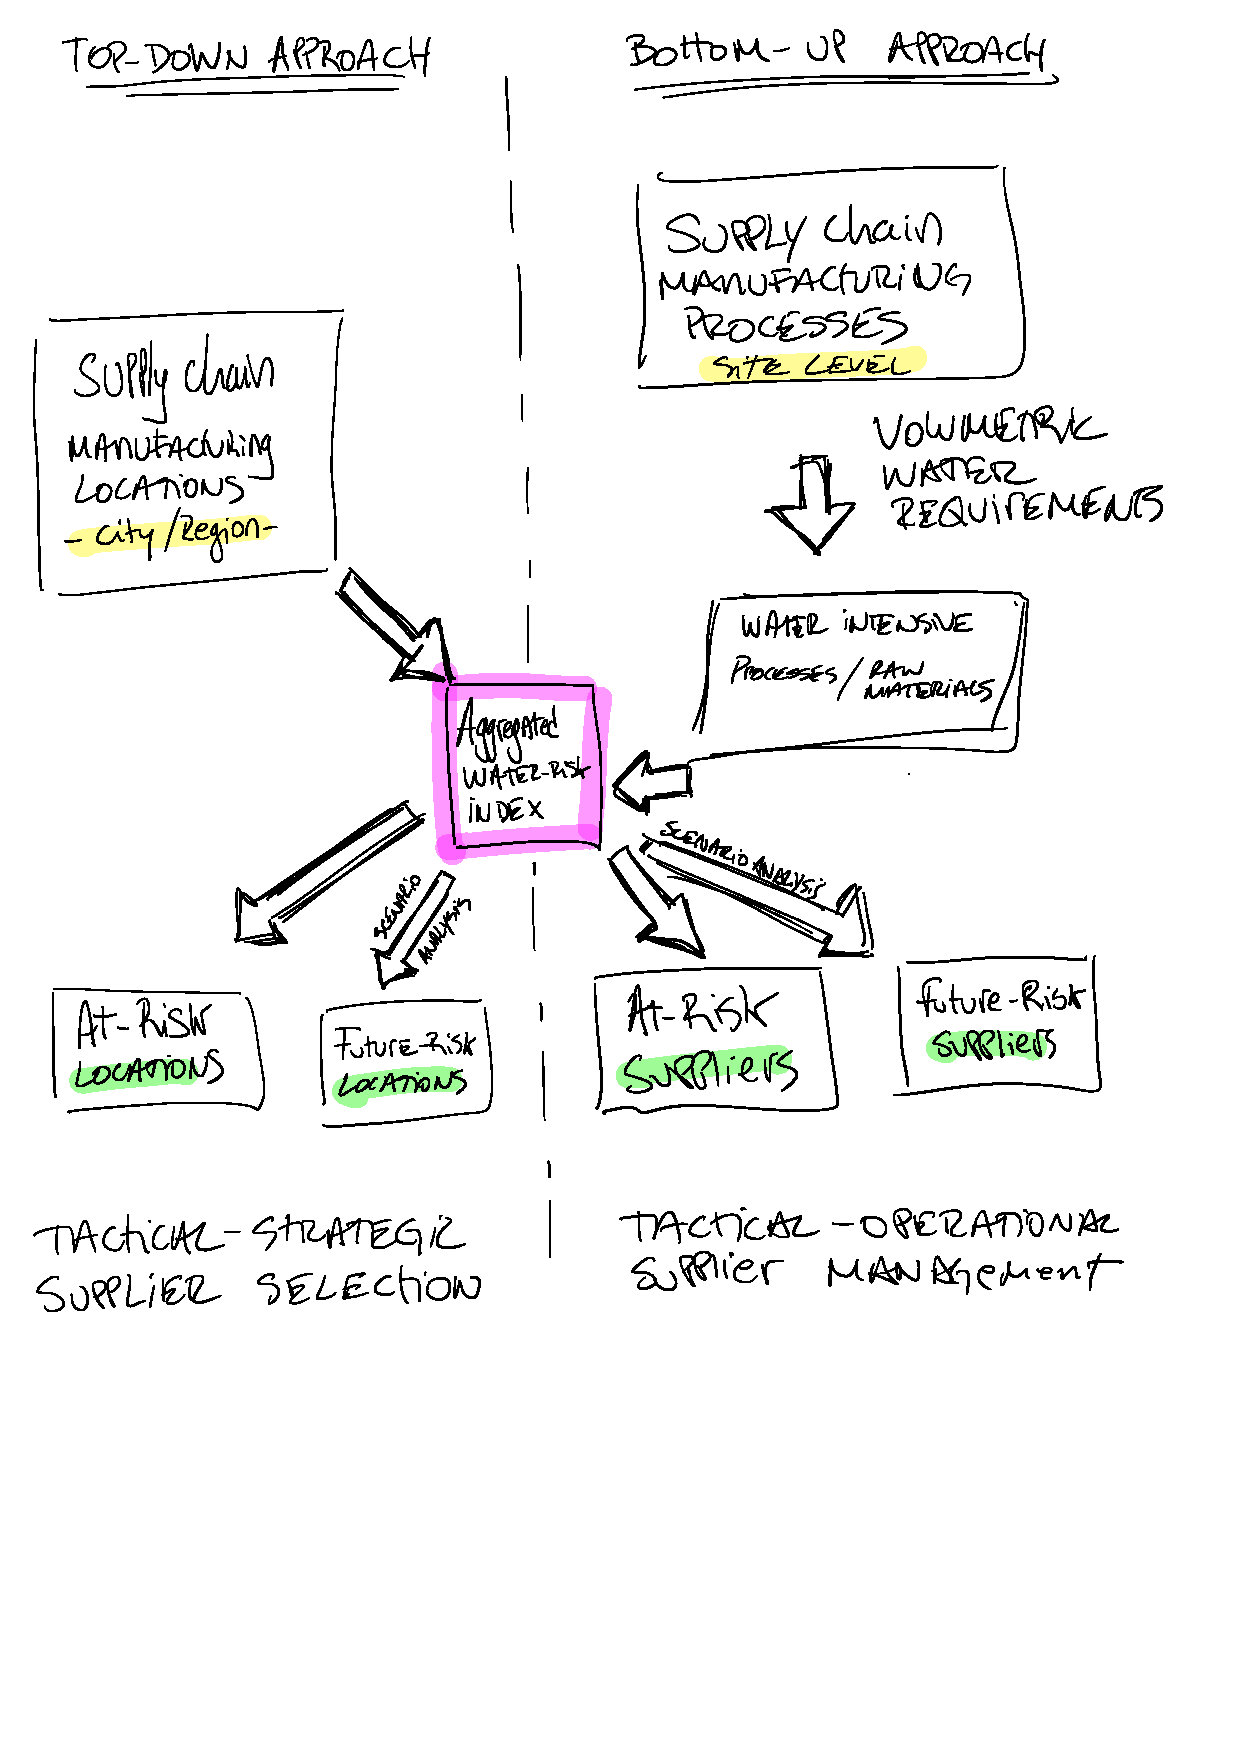
\includegraphics[ width=.7\textwidth]{plots/framework_v1.pdf}
\caption{Our water-risk screening framework.}
\small
\smallskip
\flushleft
\label{fig:framework}
\end{figure}

Central to both approaches is the aggregated supply chain water risk index.
Starting from 6 publicly available water-related measures, we use an adapted Monte Carlo Analytic Hierarchy Process (MCAHP) to construct a single index. 

In line with technical and environmental reports \citep[see e.g.,][]{Reig:2013, Orr:2011}, we recognize different mechanisms behind water risk measurement. 
Specifically, we distinguish between the direct effect on risk due to physical measurements (such as the drought severity in a particular catchment), and the amplifying effect of regulatory and reputational measurements (such as the governmental enforcement of existing regulations).

%Current methodologies suggest the use of indicators for physical water stress and regulatory or reputational water risk indicators that amplify physical water risks \citep{Reig:2013, Orr:2011}. 
%As a multinational company often has multiple decision makers with different backgrounds, the methodology needs to simplify the complexity of water risk by establishing a single aggregated index score.
%This allows everyone to speak the same “risk language” across businesses and countries. %For the screening framework we use the mentioned AHP to reach an aggregated index methodology by providing indicator weights. 
%AHP--part of MCDM--is more specifically categorized within the Multi Attribute Decision Making (MADM) methods. 


\subsection{Relevant measures of water risk} \label{sec:metrics}
%Within the categories of physical and amplifying water stress the following indicators were identified.

\subsubsection{Physical water risks}
We quantify physical water risks through the metrics of water stress, seasonal variability, and drought severity.
We obtain catchment-level data for these metrics from the World Resources Institute (WRI) Aqueduct Global Maps 2.1 dataset \citep{Gassert:2014}.

%(for baseline water stress and seasonal variability) and the \citet{Sheffiled:2008} drought dataset for drought severity.
%It focuses on areas where the actual withdrawal of water occurs by using a catchment-to-catchment flow accumulation approach. 
%This means, it aggregates water by catchment and transports it to the next downstream catchment while removing adjacent consumptive use. 
%To be able to aggregate the indicators on a comparable scale, the indicators were normalized over a set of thresholds over a five interval scale (0= no risk and 5= extreme risk). 
%Thresholds were based upon existing literature, the range and distribution of indicator values or expert judgements \citep{Gassert:2014}.
%This scaling approach is further used in this methodology for all indicators. 
%The thresholds and normalization formulas are depicted in the Appendix based on different literature and expert judgements \citep{Gassert:2013, Gassert:2014, Diop:2002}.

\begin{enumerate}
	\item Baseline Water Stress (BWS).\\
The Baseline Water Stress measures the ratio of total annual blue water withdrawal $(Ut)$ divided by the average annual available blue water $(B_a)$ for the period 1950-2010. 

\begin{align}
r_{BWS}=\frac{Ut_{2010}}{\mathit{mean}_{1950,2010}(B_a)}
\end{align}

In contrast with other water stress indicators (REF), BSW explicitly considers the accessibility of water. This is particularly relevant in resource-rich countries that have significant amounts of water available, but that are not always accessible (e.g., Brazil). 

	\item Seasonal Variability (SV).\\
Seasonal Variability quantifies the natural variation in surface water supply while ignoring human influences (e.g. diversions and infrastructure). 
Specifically, it measures the ratio of the coefficient of variation of total blue water for each calendar month $(BT_m)$ and the overall mean monthly blue water. 
\begin{align}
r_{sv}=\frac{\mathit{sd}_{jan,\dots,dec}(\bar{BT_m})}{\mathit{mean}_{(jan,\dots,dec)}(\bar{Bt_m})},
\end{align}
with $\bar{Bt_m}=\mathit{mean}_{(1950,2010)}	(Bt_{i,m})\:, m \in{jan,\dots,dec}.$

SV explicitly accounts for destabilizing climate conditions that result in large uncertainty of the water supply. 

\item Drought Severity (DS).\\
%Both of the previous indicators are measuring the blue water hydrologic cycle of water. 
Drought Severity measures relative green water availability at a certain location over a period of time \citep{Schyns:2015}.
It focuses on regions where soil moisture deficits are longer and drier, which makes it difficult to adapt to and mitigate. 
%A dataset based on \citep{Sheffield:2008} was used to show a monthly soil moisture hydrograph for different locations. 
A drought run is defined as a continuous period in which soil moisture remains below the 20th percentile of the monthly hydrograph\footnote{A graph of the water level/rate of flow of a water catchment in relation to a function of time.} $(q(\theta)<20\%)$. The severity of drought run $i$, $(S_i)$, beginning at time $t_0$ is determined by the length of the drought $(D_i)$ multiplied by its intensity $(I_i)$.
The length is measured in months, and the intensity in average number of points beneath the 20th percentile $(q(\theta))$. 
The drought severity indicator for a specific location is determined by:
\begin{align}
S= \sum_{t=t_0}^{D} (20\%-q(\theta)_t).
\end{align}
Following \citet{Gassert:2014}, we use the resampled mean drought severity data across the different hydrologic catchments, 
\begin{align}
r_{\mathrm{DRO},j}=\sum_{p\subset j} \mathit{mean}(S)_p.
\end{align}
This indicator is aggregated over a historical period of time through measuring drought events from 1901 to 2008. 
\end{enumerate}

To quantify future scenarios, we follow \citet{Luck:2015}, who developed a robust model to project baseline water stress and seasonal variability for the next 10, 20 and 30 years.
The model projects climate (i.e., supply) and socioeconomic variables (i.e., demand) to estimate the future water stress and variatbility. 
Climate variables include levels of temperature increase and constraint of emissions, whereas socioeconomic variables include population and GDP growth or level of urbanization. 
For the climate change variables, the authors assume relatively unconstrained emissions and a temperature increase of 2.6-4.8 degrees Celsius until 2100 (relative to 1986-2005 levels).

\begin{figure}
\centering
\begin{subfigure}[b]{0.31\textwidth}
                \centering
            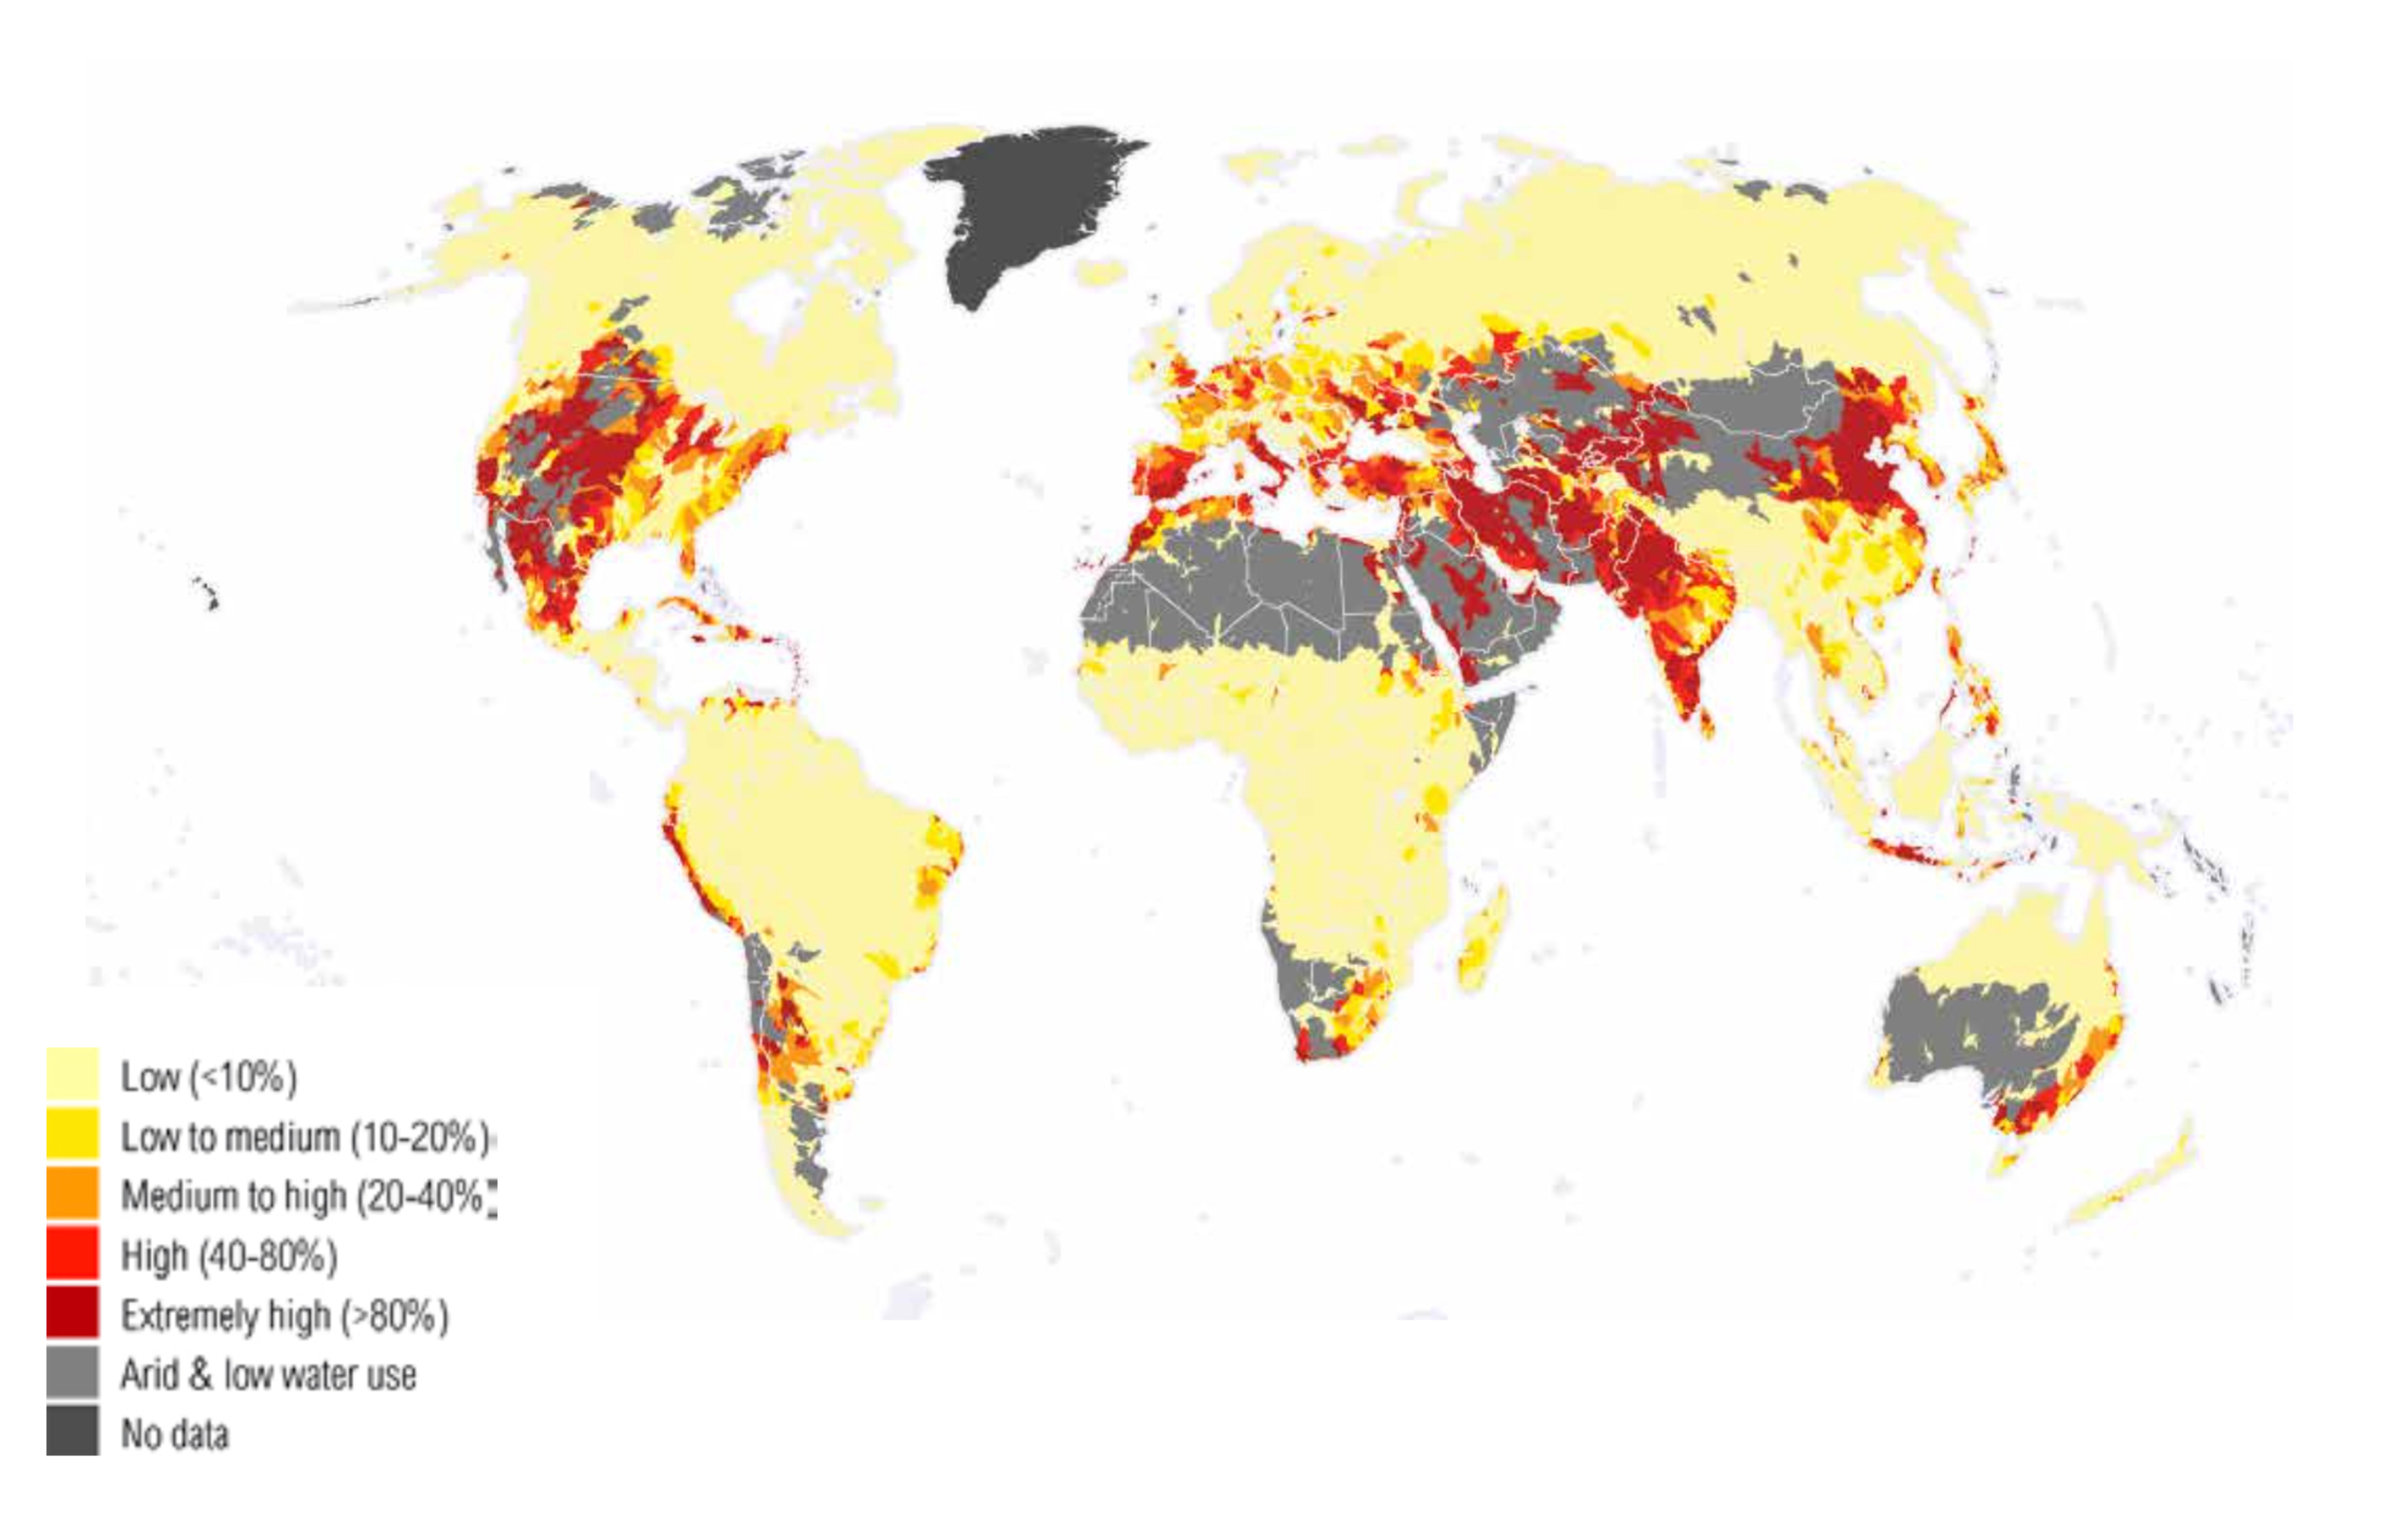
\includegraphics[width=\textwidth]{plots/bws_v1.pdf}
  \caption{Baseline Water Stress.}  \label{fig:bws}
        \end{subfigure}
\centering      
\begin{subfigure}[b]{0.31\textwidth}                  
       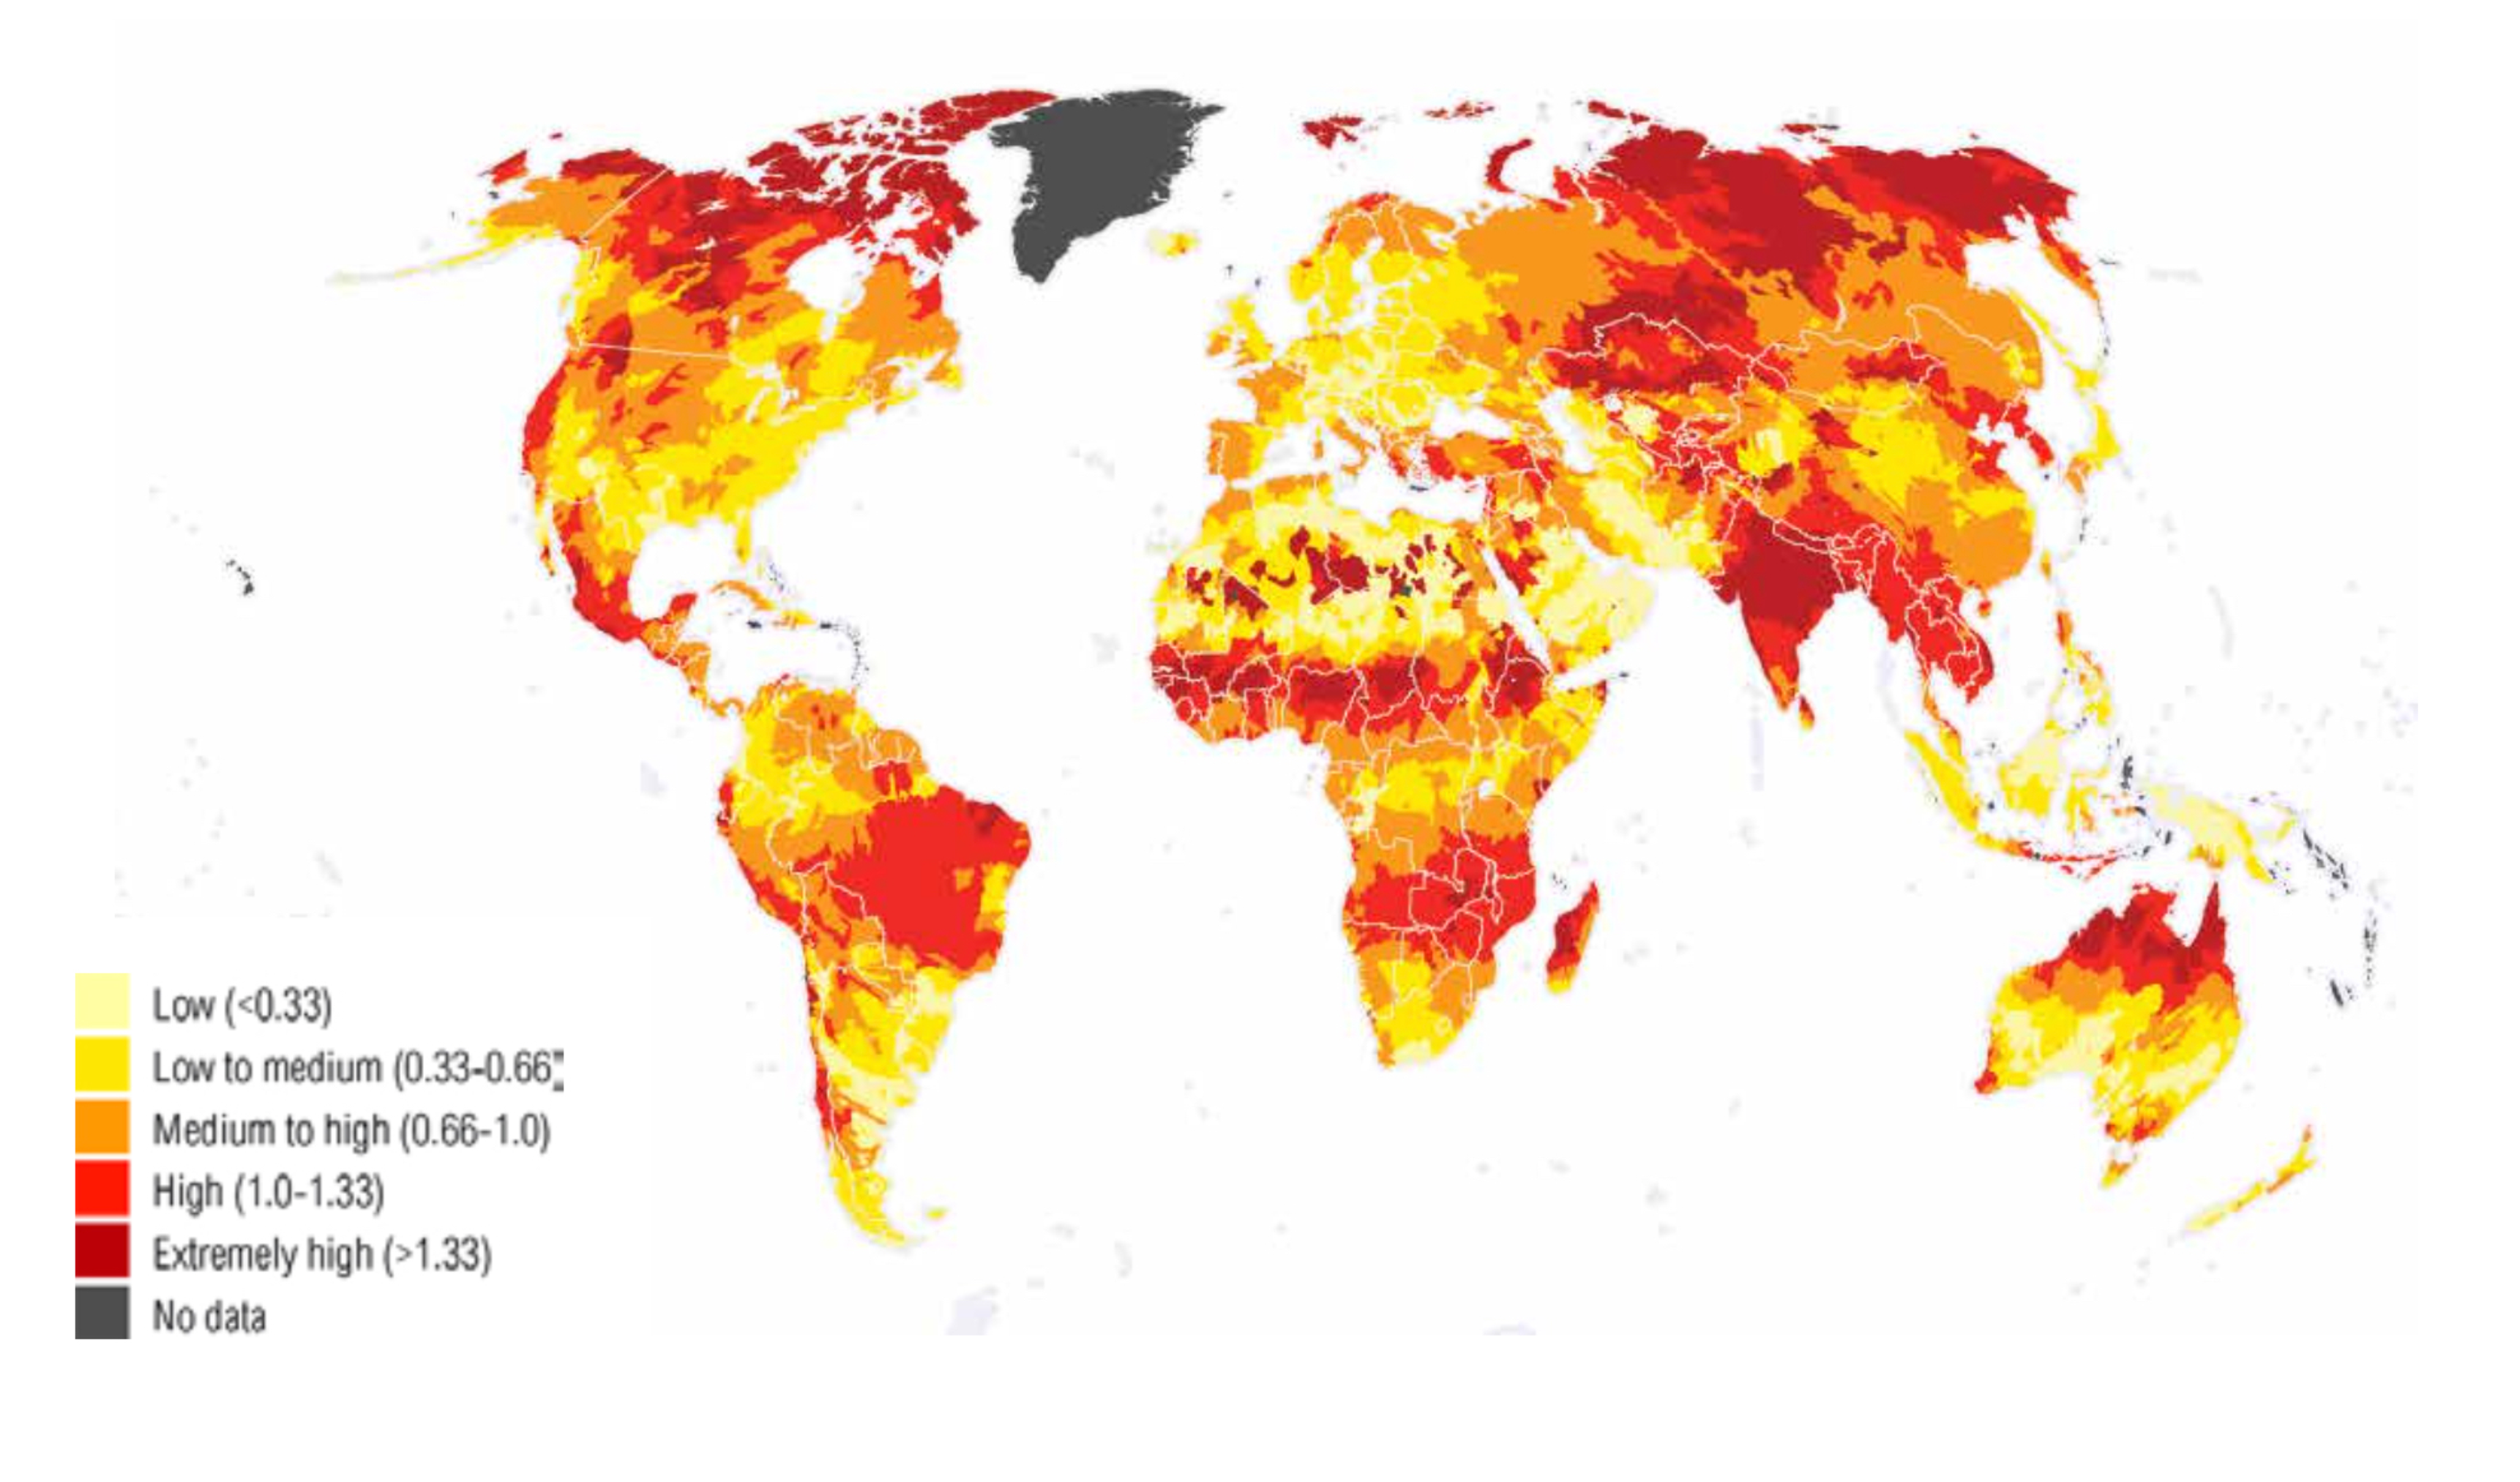
\includegraphics[width=\textwidth]{plots/sv_v1.pdf}
  \caption{Seasonal Variability.}\label{fig:sv}
        \end{subfigure}
\centering
\begin{subfigure}[b]{0.31\textwidth}                  
       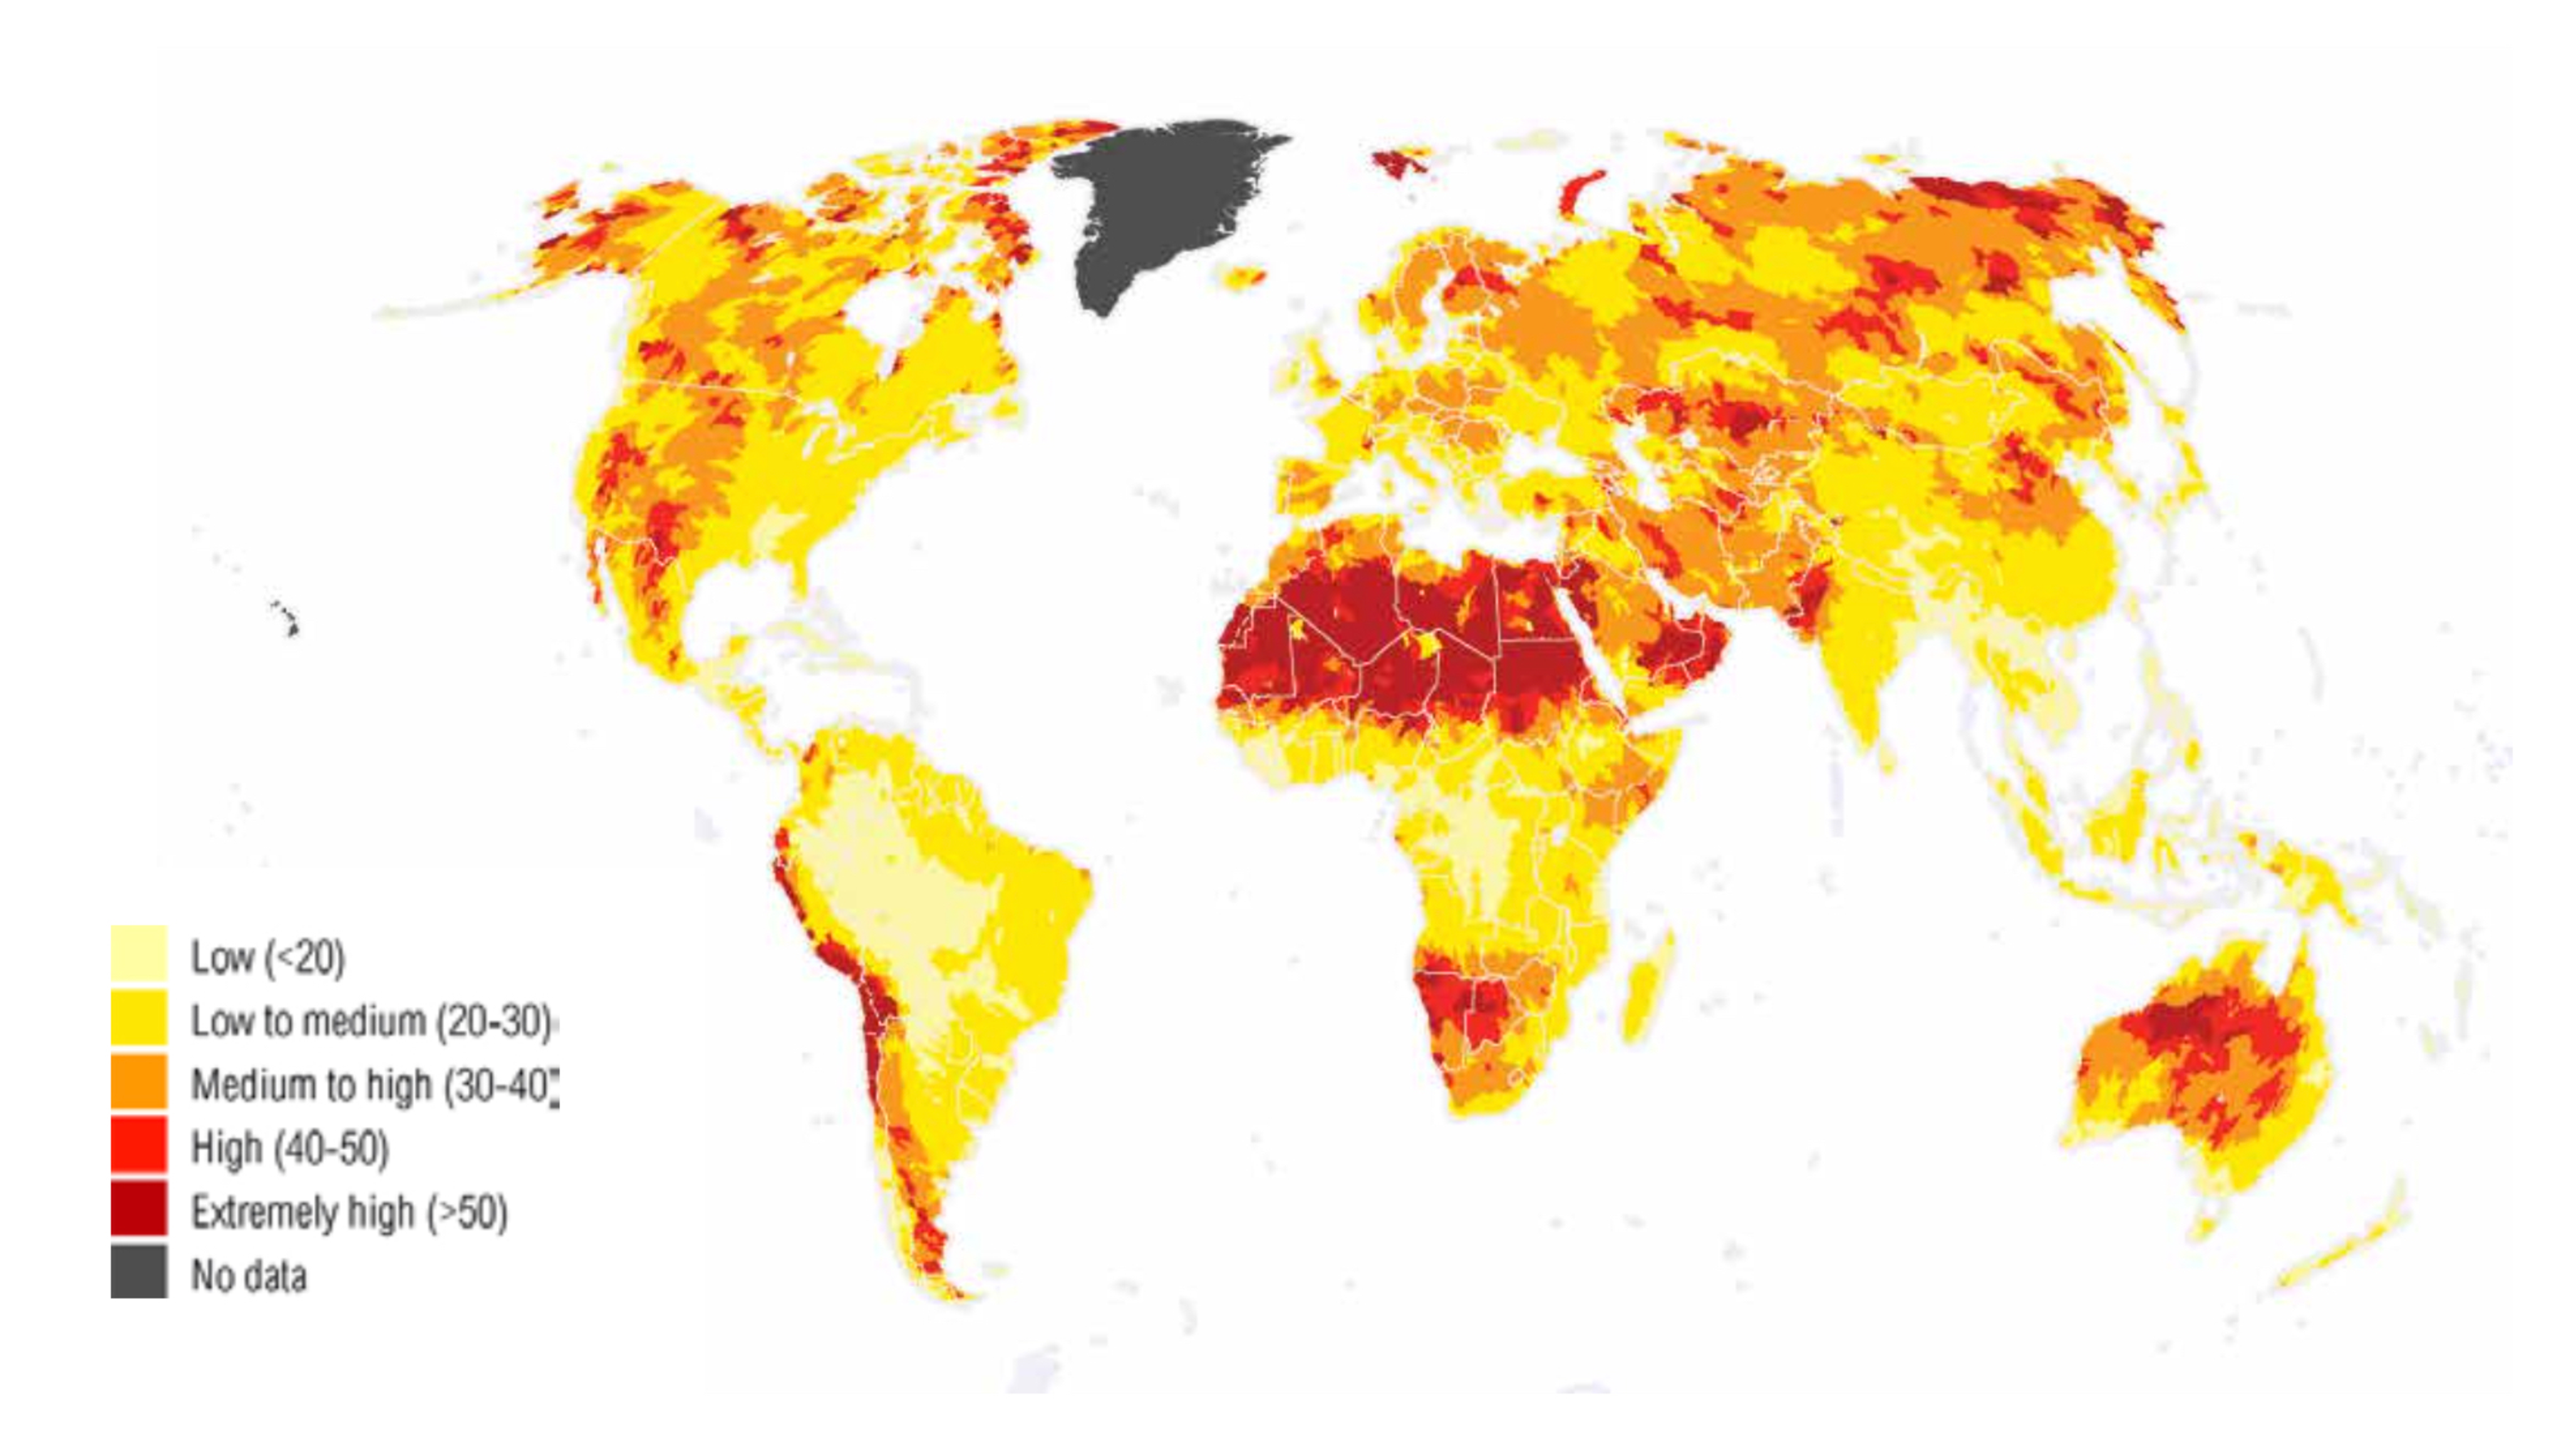
\includegraphics[width=\textwidth]{plots/ds_v1.pdf}
  \caption{Drought Severity.}\label{fig:ds}
        \end{subfigure}
\caption{Physical Water Risk Indicators (Source: WRI)}      
        \label{fig:Physical_indicators}
\end{figure}

\subsubsection{Amplifying water risk}
Water stress is not only physical, but also can be further triggered and amplified by the ecosystem such as the regulatory environment. 
We identified the following indicators on country-level to best represent amplification of water risk: External dependency; governance and regulation; and infrastructure.

\begin{enumerate}
	
	\item External Dependency Ratio (EDR).
If water is scarce, countries often rely on water imports from other countries and if high dependency on water imports exist, this can become a larger problem during scarce periods. 
The  indicator is based on the Dependency Ratio developed by the Food and Agriculture Organization of the United Nations (FAO). 
It shows the percentage of total renewable water resources originating from outside a country \citep{FAO:2016} and ranges between 0\% and 100\%. 
To scale this indicator, a linear normalization over a maximum threshold is taken. 
To determine this threshold for critical dependency, \citet{Diop:2002} proposes a percentage of 85\%. 
While this is a good indicator on external dependency, it does not show if a country exports water to other countries (hence a negative \%) which would correctly reflect additional water resources.
	
	\item Governance and Regulation (GR).
Proficient governance is of tremendous importance for local water management. 
Local, state or federal government control how water is withdrawn and then supplied to companies and other consumers. 
Moreover, regulatory institutions define taxes and prices or request specific water quality standards from companies when water is discharged. 
For this screening methodology the six Worldwide Governance Indicators (WGI) - published by the World Bank since 1996 - are chosen \citep{Kaufmann:2011}.
These indicators are based on three main signals of governance – making it a signal-extraction model approach:

	\begin{enumerate}
		\item The process by which governments are selected, monitored, and replaced.
		\item Capacity of governments to formulate effectively and implementation of sound policies.
		\item Respect of citizens and the state for the institutions that govern economic and social interactions among them.
	\end{enumerate}

The model assumes that each individual data source provides an imperfect signal of some deeper underlying notion of governance that is difficult to observe directly. 
This underlying notion suggests several smaller signals being used for different governance indicators.
 
While taking other governance indicators into consideration - such as the World Governance Indicator (WGI) (Forum for a new World Governance, 2011) or the Corruption Perception Index (CPI) - we conclude that the World Bank approach provides the most extensive methodology for governance. 
 Ranking weights according to importance for the six governance indicators was not considered due to correlation and difficulty of signaling the linkage towards concrete governance. 
 By choosing the average of the six percentile rank values for each indicator, the information used were relative ranks across all countries. 
 As a low value in the percentile ranks suggests bad governance, which is the opposite of the needed scale, we reversed the percentile ranks. 
 Afterwards, we linearized each of the six indicators on the chosen scale from 0-5, before averaging the six governance indicators. 
 	
 	\item Infrastructure (I).
Infrastructure is one of the biggest challenges facing the insecure supply of water. 
While population continues to grow extensively, water infrastructure continues to deteriorate and enormous investments and maintenance need to be made to uphold the supply of water for the public and companies. 
The OECD estimates that by 2025 the biggest share of global infrastructure investments is on water infrastructure \citep{OECD:2011}.
The World Health Organization publishes an annual dataset that tries to measure the access of public to an improved water source \citep{WHO:2016}.
It refers to the percentage of population using an improved drinking water source within a given country (e.g. piped water, public taps or rainwater collection). 
To translate this to infrastructure development indication, we observe this indicator over a period of time. 
The time period of 2000-2015 is considered and the difference to 100\% accessibility is summed up. 
For the normalization, we identified a critical threshold of 65\% of the public having access to water \citep{Diop:2002}.
This translates to a scaled value of 5 if a country provided over the last 15 years on average 65\% or less of the public with access to water.
\end{enumerate}


\begin{table}[t]
\centering
\caption{Summary of indicators}
\label{tab:inv_regression} 
\resizebox{10cm}{!} {
\begin{tabular} { l l l l l l l } 
\toprule
Indicator & Formula & Source \\
\midrule
\textbf{Physical water risks} & & \\
Baseline Water Stress & $r_{BWS}=\frac{Ut_{2010}}{\mathit{mean}_{1950,2010}(B_a)}$ & \citet{Gassert:2014} \\
Seasonal Variability & $r_{sv}=\frac{\mathit{sd}_{jan,\dots,dec}(\bar{BT_m})}{\mathit{mean}_{(jan,\dots,dec)}(\bar{Bt_m})}$ & \citet{Gassert:2014} \\
Drought severity & $S= \sum_{t=t_0}^{D} (20\%-q(\theta)_t)$ & \citet{Gassert:2014} \\
\textbf{Amplifying water risks} && \\
External dependency ratio & & \citet{FAO:2016}\\
Governance and regulation & & World Bank \\
Infrastructure & & \citet{Diop:2002}\\
\bottomrule                                                                                                                                                 
\end{tabular}
}
\end{table}
After introducing the above indicators we conducted statistical analysis through the (Pearson) correlation which showed no noteworthy correlation.


\subsection{Constructing a water-risk index}
\subsubsection{Analytic Hierarchy Process and Monte Carlo Analytic Hierarchy Process}
In this section we use Multiple Attribute Decision Making (MADM) methodologies to construct a single water-risk index based upon the physical and amplifying water risks presented in Section \ref{sec:metrics}.
In particular, we use a Monte Carlo Analytic Hierarchy Process (MCAHP, a simulation-based extension of Analytic Hierarchy Process, AHP) approach to derive weights for each of the individual metrics using survey data from expert judges.

The Analytic Hierarchy Process (AHP) methodology is broadly used as a preference theory in decision making.
Of particular relevance for this study is its extensive use in Supply Chain decision making.
(See, e.g., \citet{Ishizaka:2011} for and an application to supplier selection, and \citet{Momani:2011} for an application to xxx field.)
AHP uses independent, judgemental, pairwise comparisons among attributes to derive reciprocal comparison matrices.
Provided that these matrices pass a validity test (i.e., the comparisons made by each individual are internally consistent), a single vector of weights can be computed.

Let $A_k=[a_{kij}]$ be a positive comparison matrix.
Here, $a_{kij}$ is the judgemental evaluation of expert $k \in \lbrace 1 \dots N \rbrace$, comparing attributes $i  \in \lbrace 1 \dots m \rbrace $ and $j  \in \lbrace 1 \dots m \rbrace$.
Following \citet{Saaty:1987}, the elements of the matrix correspond to a discrete Saaty scale; $a_{kij}=\lbrace 1,\dots,9\rbrace$, where $1$ indicates no difference on the importance of attribute $i$ over $j$, and $9$ indicates the highest possible order of affirmation for the importance of $i$ over $j$.
The reciprocal elements of a comparison matrix are computed such that $a_{kji}=\lbrace \frac{1}{9},\frac{1}{8},\dots,\frac{1}{1} \rbrace$.

The entries of $A_k$ need not be transitive. 
I.e., for a given expert $k$; $a_{k12}>1$ and $a_{k23}>1$ does not imply $a_{k13}>1$.
Thus, we calculate the consistency index $(CI)$ and ratio $(CR)$ to quantify the internal validity of a matrix.
Formally, $CI=(\lambda_{max}-n)/(n-1)$, where $\lambda$ xxxx. 
A small change in $a_{kij}$ implies small changes in $\lambda_{max}$, with a small difference between $\lambda_{max}$ and $n$ being an adequate measure of consistency. 
Moreover, the consistency ratio is defined as $CR=CI/RI$, with $RI$ the random matrix consistency index, defined as the average value of $CI$ for random matrices using the Saaty scale. 
When $CR$ is less than or equal to 0.1, the comparison matrix is considered to have an acceptable consistency \citep{Ishizaka:2011, Saaty:1987}.

MCAHP incorporates Monte Carlo simulation into the AHP methodology.
Rather than computing the required weights from the comparison matrices, these are used to estimate a continuous distribution for each pairwise comparison.
MCAHP, thus, addresses the uncertainty inherent in decision makers required to translate 
subjective judgements into a single point estimate \citep{Ataei:2013}.
In addition, MCAHP allows for statistical sensitivity analysis of the results \citep{Banuelas:2004, Vaidya:2006}. 

%With MCAHP, Instead of using discrete values for each pairwise comparison, a continuous distribution derived from the multiple expert matrices is used and simulated. 
%For distributions, other research studies considered for example uniform \citep{Hauser:1996} or triangular distributions \citep{Banuelas:2004}.
%Whereas a uniform distribution assumes a very large variance in judgements, the triangular distribution considers minimum, maximum and most likely values. 
%Such approaches take into consideration the uncertainty that decision makers have when they are forced to converge subjective judgements to a single point estimate. 
%With the use of simulation, it is assumed that higher levels of confidence can be reached by achieving a large number of consistent matrices that were derived from the distributions of the collected pairwise comparisons \citep{Hauser:1996}.
%
%To allow for uncertainties, while having a small sample size of experts $(N=11)$,  we took an adjusted simulation approach based on MCAHP which has also been use by other research studies \citep{Hauser:1996, Ataei:2013}.
%With this approach we find a best fit of distribution for each array $a_{kij}$. 
%While this violates the concept of the AHP methodology - also resulting in a wider spread of inconsistencies – we allow for better fit distributions depicting the actual made judgements and not relying solely on the derived distributions of one triangular of all the matrices. The fit of distribution functions for the arrays was found through the Kolmogorov-Smirnov (K-S) test– a Goodness-of-Fit Test (GoF). 
%The test is most viable due to its applicability on small sample sizes without any restrictions \citep{Romeu:2003, Babu:2006}. For robustness, the MCAHP approach by \citet{Ataei:2013} was also simulated, but the adjusted approach reached a higher number of consistent matrices and a lower average consistency index in all 30 conducted simulation with each 10,000 iterations. 

\subsubsection{Judgemental Comparisons and Resulting Index}
Based on the adapted simulation MCAHP approach, we fit the distributions, derive the K-S test, and run the Monte Carlo Simulations. 
 For the K-S test, the critical value of $D_n$ with a high significance level of $\alpha=0.2$ was $0.307$.


\begin{table}
\caption{Resulting indicator weights}
\centering
%\resizebox{7cm}{!} {
\begin{tabular} {p{4cm} l l} \\ 
\toprule
	 &	\multicolumn{2}{l}{Adapted MCAHP approach} \\
\midrule 	
Number of consistent matrices (mean/median) & \multicolumn{2}{c}{1095.33/1100.5}\\
Consistency index							& \multicolumn{2}{c}{0.06}\\
Indicator									& Mean & StdDev\\
BWS											& 44.28 \% 	& 5.13\% \\
SV											& 22.97\% & 4.72\%\\
DS	& 11.64\% & 3.68\%\\
EDR	& 8.30\%  & 2.91\%\\	
GR 	& 6.25\%  & 2.07\%\\
I	& 6.56\%  & 2.23\%\\
\bottomrule
\end{tabular}
%}
\end{table} 

As mentioned, also the geometric mean and the simulation approach of \citep{Ataei:2013} were conducted.
For none, the order of the indicators changed and the adapted approach showed the most confident results while enabling the consideration of uncertainty.
In conclusion, the three highest weighted indicators BWS, SV, and DS make up $78.89\%$ of the weights. 
The amplifying indicators--GR, I, and EDR--account for $21.11\%$  (at a country-level). 
These weights were vetted afterwards with a selected group of internal and external experts.


\section{Application and Results}
\subsection{Data}
%We use data from xxx consumer good categories. 
%This (these?) product(s) is characterized by xxx. 
%This is a picture of the supply chain, bla bla.
The methodology was applied in two ways within the context of the complex supply chain of a multinational consumer goods company. 
The first was a top-down approach to enable the prioritization of suppliers on the basis of water risk. 
The second was a bottom-up application in combination with a Life Cycle Assessment (LCA) water consumption methodology to analyse a water-intense raw material group and the locations of the suppliers based on their site-related water risk. 
Both applications provide an efficient and robust way to arrive at actionable results for a multinational company with a complex and wide-reaching supplier network.
 
 INCLUDE SUMMARY STATISTICS ON THE DATASET
 
\subsection{Top-down Approach}
%We use the data to aggregate the water risk at the level of individual manufacturing locations and countries/regions.
%We show that there is a considerable variability among countries, but also among particular suppliers. 
%This indicates that some countries need to be prioritized in the analysis because they are too dirty and/or they are very sensitive (i.e., huge difference among suppliers).
A sample of 1,066 suppliers located in four regions was investigated using the top-down application of the methodology in order to identify supplier locations experiencing the highest water risk. 
Overall, Asia was identified as the region where suppliers are currently experiencing the highest water risk, followed by Europe, Middle East and Africa (EMEA), Latin America (LA), and North America (NA).
 With the inclusion of the future water stress projection of \citet{Luck:2015}, the percentage of suppliers with high water scarcity risk scores $(>2.5)$ was projected to increase across all four regions by 2040. 
 The results of the aggregated water risk index allowed for the identification of 370 at-risk suppliers for prioritization. 
 
After narrowing the list of at-risk suppliers to less than 35\% of the original scope using the aggregated water risk index, an additional layer of assessment was introduced to allow companies to consider the social aspects of water risk alongside the environmental aspects, as advocated by Sustainable Development Goal (SDG) 6.  
This was done by including the improved water source and sanitation (access to water) indicator \citep{WHO:2016}. 
The critical threshold was set to 90\%.  
As this indicator was the foundation for the proxy infrastructure development indicator in the aggregated index, we found a highly significant correlation of 0.95 (p-value $< 0.001$). 
Thus, the decision was made for this specific application to exclude the infrastructure indicator from the aggregated water risk index in the top-down application of the methodology so as to not xxxx...

All material suppliers were grouped by country and plotted in a graph. 
The size of the circle indicates the total annual spend on suppliers located within the country. 
The error bars show the range of aggregated water risk index scores of the suppliers within each country.
 In many cases, the scores vary greatly between suppliers within a single country (e.g. India). 
 This again emphasizes the local nature of water issues that can change drastically across geographies.
 Suppliers of most concern were in the upper right quadrant (red zone), which meant that they were located in regions of high-very high water risk $(>2.5)$ and were operating in countries where less than 90\% of its people have access to improved water and sanitation sources. 
 A significant number of suppliers within Peru, Indonesia, and Morocco lay within this high risk quadrant. 
 Based on the two dimensions, this top-down application enabled the identification of 14 at-risk suppliers for recommended prioritization from the original list of over 1,000 suppliers.

INSERT PLOTS HERE. THE ONES IN THE WORD FILE PLUS THE LITTLE MAPS.

\begin{figure}
\centering
\begin{subfigure}[b]{0.45\textwidth}
                \centering
            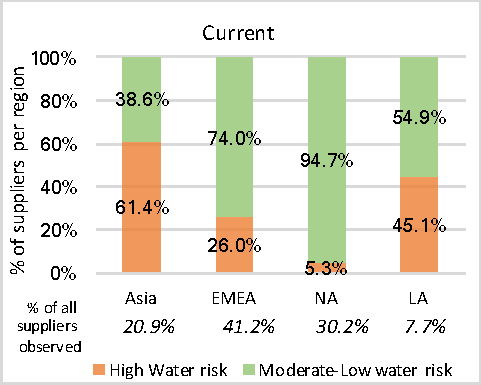
\includegraphics[width=\textwidth]{plots/water_risk_now_v1.pdf}
  \caption{Current water risk per region.}  \label{fig:water_risk_now}
        \end{subfigure}
\centering      
\begin{subfigure}[b]{0.45\textwidth}                  
       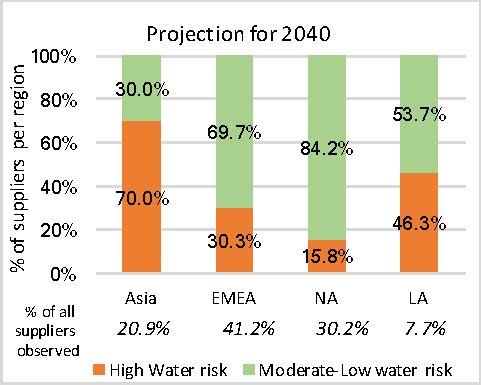
\includegraphics[width=\textwidth]{plots/water_risk_future_v1.pdf}
  \caption{Expected water risk per region.}\label{fig:water_risk_future}
        \end{subfigure}
\caption{Water risk}      
        \label{fig:water_risk}
\end{figure}

\begin{figure}[t]
\centering
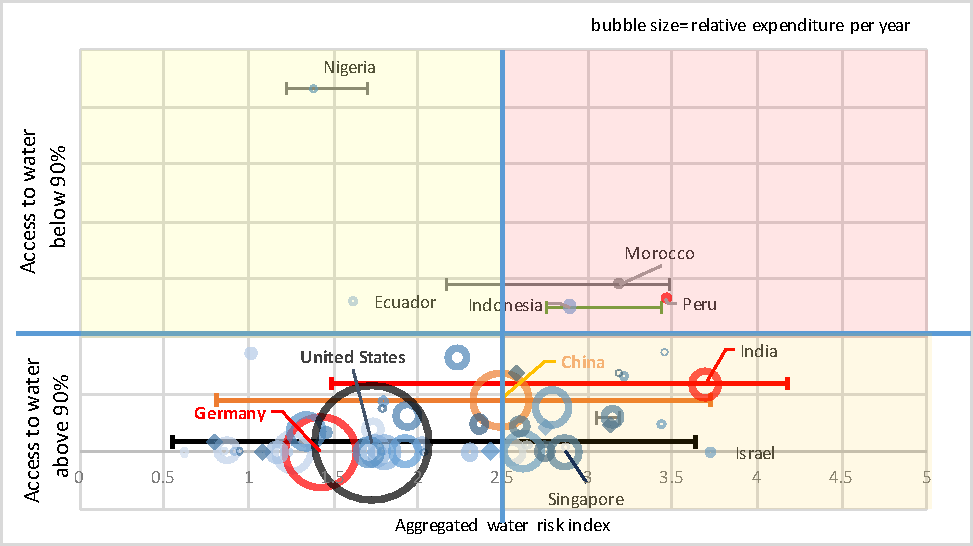
\includegraphics[ width=.7\textwidth]{plots/top_down_results_v1.pdf}
\caption{Water risk analysis for all suppliers.}
\small
\smallskip
\flushleft
\label{fig:top_down_results}
\end{figure}

\subsection{Bottom-up Approach}
%We use the data to consider the case of an individual raw material. 
%We analyze the different tradeoffs inherent in the choice of different suppliers. 
%etc.

INCLUDE THE ANALYSIS OF THE WATER-INTENSITY OF THE RAW MATERIALS

This application demonstrates the capability of the methodology to use water consumption methodologies (LCA \& WFA) in combination to determine water risk at supplier locations. 
Within water footprint and water risk research, such a combined application was not found before the completion of this study. 
This work and accompanying results highlights the need to include the water consumption of individual suppliers in combination with water risk results in order to get a more holistic understanding of risk at the site level.
The water use data was given directly to the multinational company by the suppliers in scope and was complemented by the water background flow data from LCA databases. 
With water risk and water consumption making up the first two dimensions, the purchased raw material amount formed the third in order to account for dependency of the organization on the supplier. 
The future water projections were also reflected within the graph (dotted line circle) to depict the predicted conditions for water risk in 2040.
All supplier locations were below high risk levels (threshold $>2.5$ for aggregated water risk index).
 However, Supplier 3 was the largest raw material purchase source of all four active suppliers and was located in a medium risk region. 
 Due to supplier dependency and the fact that the site is on the threshold of high water risk, the recommendation was made to engage with Supplier 3 and learn more about what is being done there to minimize the water risk.

\begin{figure}[t]
\centering
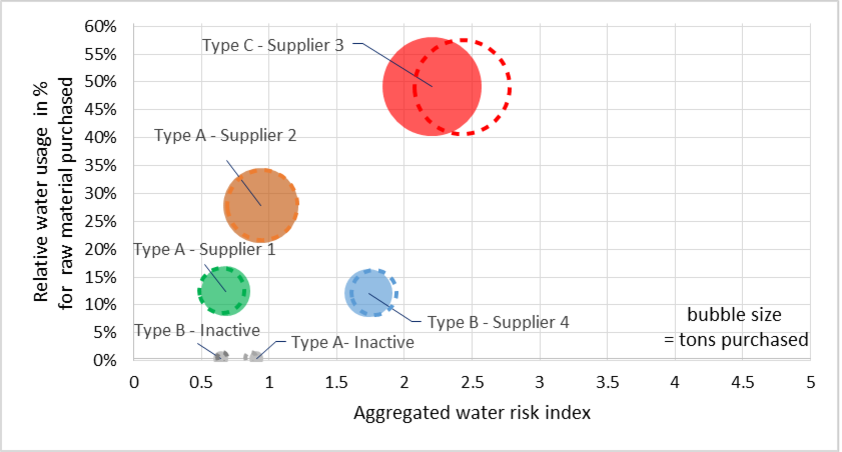
\includegraphics[ width=.7\textwidth]{plots/bottom_up_results_v1.pdf}
\caption{Water risk analysis for xxx raw material.}
\small
\smallskip
\flushleft
\label{fig:bottom_up_results}
\end{figure}
 
\section{Conclusions}
%We advanced the theory in such a way because we xxx.
%From a managerial perspective, our study introduces a new way to quantify the water risk dimension within the framework of supplier selection. 
%We demonstrated the operational use of our methodology in the case of analyzing different producers of a given raw material, and its tactical use in analyzing the water risk associated with a firms' suppliers at a country level in terms of mean risk as well as variability/uncertainty.
%
%Our study has a number of limitations. 
%(1) We still rely on qualitative data. 
%(2) The data is very difficult to retrieve.
%
%We see two further areas of study. 
%(1) Refining and/or validating the indexing/weighing mechanism for the different measures, (2) something else. 
The novel development of a multiple-indicator water risk methodology for use in the assessment of water risk at supplier locations helped provide a strategic, data-based approach to prioritize suppliers with respect to water stewardship interventions. 
The top-down application enabled an efficient yet robust method to screen over 1,000 suppliers to reach a short-list prioritized for further engagement and investigation. 
Any organization that knows the location of their supplier manufacturing facilities can quickly determine which suppliers they should engage with first. 
The results are immediately actionable and enable a data-based conversation to occur with the high risk suppliers. 
In addition, the methodology incorporates both environmental and social aspects of water risk, as encouraged by SDG 6. 
The bottom-up application of the methodology on a water-intense raw material group combined the results of the aggregated water risk index with water usage to better understand risk of an important raw material.  
While it is more challenging to obtain accurate water usage volumes from suppliers, the incorporation of this usage data is essential to more holistically assess risk at a supplier location. 
Without fully understanding how water is used at a facility, it is difficult to accurately assess risk.
 There may be instances when a facility is located in a high water risk region, but does not use water.
  When water usage data is not available, it is recommended to use the top-down approach of the methodology and to engage with the high risk sites to learn more about their water usage. 
This methodology can and should be used by companies to assess and act on risks related to water in their supply chain. 
  Using best available data and country-level, or sub-national metrics when available, it is possible to prioritize suppliers and supplier sites for further investigation and intervention. 
  By better understanding both the environmental and social water risk, companies will be more prepared for maintaining an efficient and effective business while being good stewards of the water they are associated with throughout the life cycle of their products and services.


\bibliographystyle{apalike}
\bibliography{references_water}

\end{document}